\begin{pastexam}[label={px:ntut-115-ee-ds-17}]{北科大電機所（戊組）115 學年度 簡答題第 2 題}
（簡答）

Given a binary search tree with root 45, and the following nodes: 25, 65, 15, 35, 55, 75, 10, 20.
Insert 18, 30, 50, 70 (in this order) into the binary search tree. What is the pre-order traversal?
\textbf{(4\%)}
\end{pastexam}

\begin{pastsoln}
答案：45, 25, 15, 10, 20, 18, 35, 30, 65, 55, 50, 75, 70。

題目沒有畫出原本的樹，下面照「根 $45$，再依序插入 $25, 65, 15, 35, 55, 75, 10, 20$」建樹（這個順序正好是一層一層
列出來的，建出來的樹最自然）：$25$、$65$ 是根的左右子節點；$15$、$35$ 是 $25$ 的子節點；$55$、$75$ 是 $65$ 的子節點；
$10$、$20$ 是 $15$ 的子節點。

再插入（資結書第~9.2~節，小往左、大往右）：
\begin{itemize}
\item $18$：$18 < 45$ 左，$18 < 25$ 左，$18 > 15$ 右，$18 < 20$ 左，成為 $20$ 的左子節點。
\item $30$：$30 < 45$，$30 > 25$，$30 < 35$，成為 $35$ 的左子節點。
\item $50$：$50 > 45$，$50 < 65$，$50 < 55$，成為 $55$ 的左子節點。
\item $70$：$70 > 45$，$70 > 65$，$70 < 75$，成為 $75$ 的左子節點。
\end{itemize}
\begin{center}
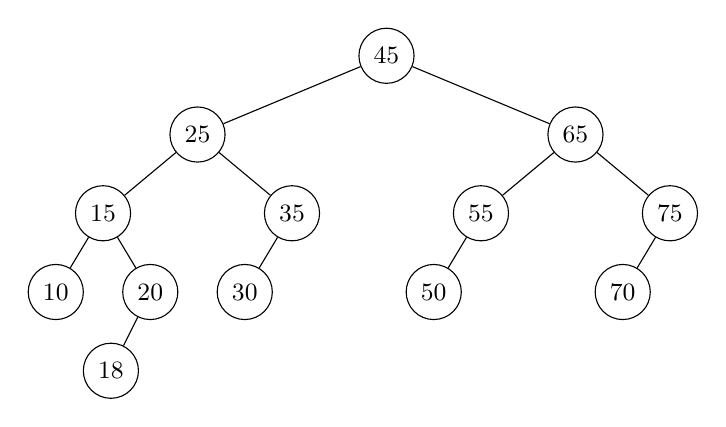
\begin{tikzpicture}[level distance=10mm,
  every node/.style={circle,draw,minimum size=7mm,inner sep=0pt,font=\small},
  level 1/.style={sibling distance=48mm}, level 2/.style={sibling distance=24mm},
  level 3/.style={sibling distance=12mm}, level 4/.style={sibling distance=10mm}]
\node {45}
  child {node {25}
    child {node {15} child {node {10}} child {node {20} child {node {18}} child[missing]}}
    child {node {35} child {node {30}} child[missing]}}
  child {node {65}
    child {node {55} child {node {50}} child[missing]}
    child {node {75} child {node {70}} child[missing]}};
\end{tikzpicture}
\end{center}
前序是「根、左子樹、右子樹」：根 $45$；左子樹 $25$ 為根，先 $25$，再它的左子樹 $15, 10, 20, 18$，再右子樹 $35, 30$；
最後右子樹 $65, 55, 50, 75, 70$。 合起來就是上面的答案。 （中序是 $10, 15, 18, 20, 25, 30, 35, 45, 50, 55, 65, 70, 75$，
遞增，可以拿來檢查樹建得對不對。）
\end{pastsoln}
